\documentclass[11pt, a4paper]{article}
\usepackage{fontspec}
\usepackage[left=3cm,right=2cm,top=2.5cm,bottom=2.5cm]{geometry}
\usepackage{polyglossia}
\setdefaultlanguage[spelling=new]{german}
\usepackage{parskip}
\usepackage{anyfontsize}
\usepackage{graphicx}
\usepackage{xcolor}
\usepackage{subfig}
\usepackage{fancyhdr}
\usepackage{hyperref}
\usepackage{titlesec}
\lhead{} \chead{} \rhead{} %sets header left center right
\lfoot{} \cfoot{} \rfoot{\thepage} %sets footer left center right
\renewcommand{\headrulewidth}{0.0pt} %optional horizontal rule thickness
\renewcommand{\footrulewidth}{0.0pt} %optional horizontal rule thickness
\pagestyle{fancy}
\usepackage{background}

\setromanfont{IBMPlexSans}[
    Path=../../fonts/,
    Extension = .ttf,
    UprightFont=*-Regular,
    BoldFont=*-Bold,
    ItalicFont=*-Italic,
    BoldItalicFont=*-BoldItalic
]

\newfontfamily\Buenard{Buenard}[
    Path=../../fonts/,
    Extension = .ttf,
    UprightFont=*-Regular,
    BoldFont=*-Bold
]

\titleformat*{\section}{\Buenard\Huge\bfseries}
\titleformat*{\subsection}{\Buenard\LARGE\bfseries}
\titleformat*{\subsubsection}{\Buenard\Large\bfseries}
    
\backgroundsetup{
scale=1,
angle=0,
contents={\ifnum\value{page}=1
\includegraphics[width=\paperwidth,height=\paperheight]{../assets/gradient@2x-t.png}\fi}
}

\definecolor{eastern}{rgb}{0.1373,0.6157,0.6784}
\newcommand{\gender}{\raisebox{-.25em}{*}}
\let\oldsection\section
\renewcommand\section{\clearpage\oldsection}

\usepackage{tabto}

\renewcommand{\glossary} {\marginsymbol{\textbf{↪}}}
\newcommand{\cited}[1]{\marginsymbol{\textbf{↗} #1}}
\newcommand{\marginsymbol}[1] {\protect\marginsymbolhelper{#1}}
\newcommand{\marginsymbolhelper}[1] {\tabto*{-1cm}\makebox[0cm]{#1}\tabto*{\TabPrevPos}}
     
\begin{document}
\raggedright
\pagecolor{eastern}
\pagenumbering{gobble}
\mbox{}
\vfill
{
\color{white}
\LARGE
\textbf{\Buenard\fontsize{50}{60}\selectfont typst}
\vspace{1cm}

\textbf{Kommentierter \\ Business Model Canvas}

{
\Large
Businessplan-Wettbewerb \\
Berlin Brandenburg 2022 

15. Februar 2022
}
\vspace{2.25cm}
}
\section*{Übersicht}
\pagecolor{white}
\pagenumbering{arabic}
\NoBgThispage
\vspace{2mm}

Typst ist ein Software-Unternehmen, das ein gleichnamiges Textsatzsystem als Software-as-a-Service-Web-App entwickelt. Die Typst-Software ist mehr als ein einfaches Textverarbeitungsprogramm: selbst Dokumente mit komplexen Layouts können einfach gestaltet werden. Dabei wird jedes Element, bis hin zum einzelnen Buchstaben, automatisch präzise platziert.

Prinzipien und Methoden des Textsatzes und der Typographie zeigen auf, wie Ideen und Informationen effektiv in Schriftform kommuniziert werden können. Deshalb sind Menschen und Unternehmen der verschiedensten Gebiete auf hochwertigen Textsatz angewiesen:
\begin{itemize}
    \item Studierende und Wissenschaftler\gender{}innen schreiben Forschungsartikel, in denen sie neue Ideen, oft mit mathematischen Formeln, visuell eingängig darstellen
    \item Verlage veröffentlichen Buchreihen mit unterschiedlichen, wiedererkennbaren Layouts
    \item Zeitungen arrangieren eine große Anzahl von Artikeln pro Seite ansprechend
    \item Unternehmen geben gedruckte Werbematerialien wie Kataloge heraus
\end{itemize}

Die bestehenden Lösungen für diese Anwendungszwecke haben alle klare Schwächen: Textverarbeitungssysteme wie Word besitzen nicht die nötige Ausgabequalität und Funktionsvielfalt für anspruchsvolle Anwendungszwecke. Professionelle Textsatzsysteme wie Adobe InDesign sind teuer und haben keine Funktionen für die durch Remote-Work immer bedeutsamer werdende synchrone Zusammenarbeit im Team. Das in der Wissenschaft verbreitete \glossary markupbasierte Satzsystem LaTeX ist langsam und schwer zu erlernen.

Bei Typst sind alle diese Nachteile eliminiert. Typst baut mit einfach anzuwendenden und austauschbaren Layoutvorlagen auf den Stärken bisheriger Systeme auf. Damit steigert es die Effizienz seiner Nutzer\gender{}innen und kann langfristig die zersplitterten Kundensegmente der Konkurrenzprodukte auf sich vereinen. Typst ist dafür designt, möglichst ressourcenschonend zu arbeiten, und ist somit nachhaltiger als bestehende Lösungen.

Zunächst wollen wir mit Typst im Wissenschaftsbereich starten. Mit \cited{1} 2,6 Millionen veröffentlichten Forschungsartikeln pro Jahr (2018) sowie zahllosen Abschlussarbeiten und Hausaufgaben gibt es einen großen Bedarf. Insbesondere in den MINT-Fächern wird hierfür bisher oft das Textsatzsystem LaTeX genutzt, das ein ähnliches Grundprinzip hat, aber für seine umständliche Bedienung bekannt ist.

Das Geschäftsmodell des Unternehmens baut auf dem Freemium-Prinzip auf: Ein Basis-Zugang zu Typst ist kostenlos verfügbar, jedoch funktional eingeschränkt. Mit einem Abonnement zu 10 € monatlich erhält die\gender{} Nutzer\gender{}in dann Zugriff auf alle Funktionen. Die Kundenbeziehungen von Typst sind darauf ausgelegt, Nutzer\gender{}innen zu helfen, Typst möglichst vielfältig einzusetzen. Zufriedene Kund\gender{}innen nutzen Typst intensiver und haben somit einen höheren Anreiz, ein Abonnement abzuschließen.

Das entwicklungsintensive Gründungsvorhaben wird durch Laurenz Mädje und Martin Haug getragen, beide kurz vor dem Informatik-Master-Abschluss an der TU Berlin und bereits erfahren in sowohl systemnaher als auch Web-Entwicklung. Das Gründungsteam wird in Kürze durch ein drittes Mitglied mit Business-Development-Schwerpunkt ergänzt.

Dieses Dokument ist mit einer frühen Version von Typst gesetzt.

% TODO Legende

\section*{Was?}
\subsection*{Wertangebot}

Unser Produkt \emph{Typst} ist ein innovatives Typographiesystem. Darunter versteht man grundsätzlich eine Software, mit der man Print-Artikel wie Bücher, Magazine und Artikel schreiben und professionell gestalten kann. Typst besteht dabei aus zwei Teilen:

\begin{enumerate}
    \item Einer flexiblen \glossary Markupsprache. In einer solchen Sprache gibt die\gender{} Nutzer\gender{}in den Inhalt ihres\gender{} Dokuments ein (wie in eine herkömmliche Textdatei) und schreibt anschließend einfache Kommandos in die selbe Datei, um das Aussehen des Dokuments anzupassen.
    \item Einer benutzerfreundlichen Web-Anwendung. Sie unterstützt die\gender{} Nutzer\gender{}in mit sofortigen Vorschauansichten, hilfreichen Bedienelementen und Autovervollständigung beim Schreiben der Typst-Markupsprache. Außerdem kann hier mit anderen Nutzern an einem Dokument zusammen (kollaborativ) gearbeitet werden.
\end{enumerate}

Die Wettbewerber des Produkts lassen sich in drei Kategorien einteilen: Andere markupbasierte Textsatzsysteme, Textverarbeitungen und graphische Desktop-Publishing-Systeme (DPS).

\begin{figure}[h]
    \centering
    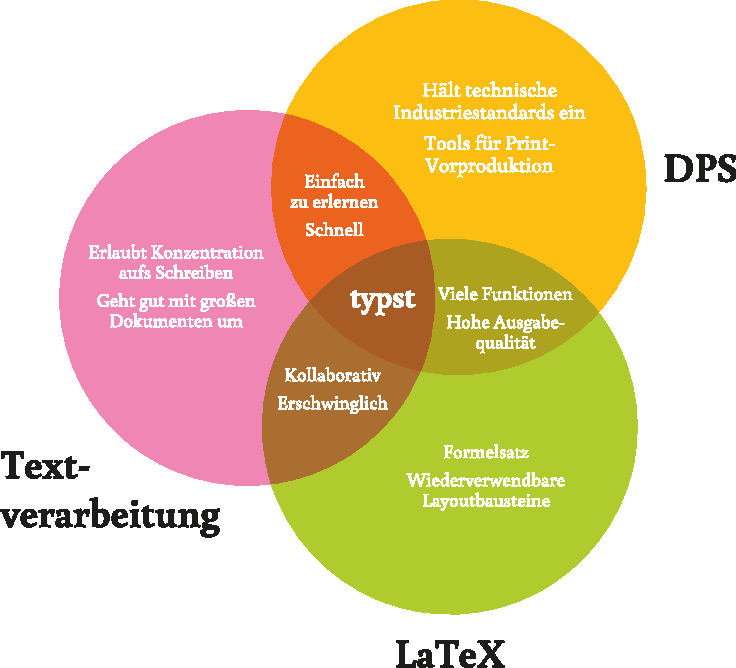
\includegraphics[width=.5\textwidth]{../assets/venn.pdf}
    \caption{Übersicht über die Konkurrenz und deren Ausrichtung.}
\end{figure}

Textverarbeitungen wie Word, Google Docs oder Apple Pages sind einfach zu lernen, jedoch fehlen ihnen viele Funktionen für professionellen Satz, teils bewusst im Sinne der Einfachheit. Dadurch leidet die Ausgabequalität. Typst hingegen bietet alle diese Funktionen -- ohne Einsteiger damit zu überwältigen.

Das einzige weit verbreitete markupbasierte Textsatzsystem ist bisher LaTeX, eine frei erhältliche und quelloffene Software, die ihre Wurzeln im Jahr 1978 hat. Darauf aufbauend ermöglicht der Online-Dienst Overleaf, zusammen an LaTeX-Projekten zu arbeiten. Typst hebt sich von LaTeX und Overleaf ab, in dem es deutlich performanter und einfacher zu erlernen ist: Zum einen sieht man die Auswirkung einer Änderungen sofort, anstatt bis zu 15 Sekunden warten zu müssen. Zum anderen muss die\gender{} Nutzer\gender{}in viel weniger lernen, um ihr\gender{} erstes Dokument zu erstellen.

Während für Desktop-Publishing-Software wie Adobe InDesign oder QuarkXPress die hohe Ausgabequalität im Fokus steht, ist bei diesen Systemen die Zusammenarbeit am gleichen Dokument schwierig, ohne E-Mails mit zum Teil veralteten Dateien umherzusenden. Synchrone Zusammenarbeit ist unmöglich. Außerdem sind diese Systeme teuer.

\subsubsection*{Kundenbedürfnisse}


\textbf{Vielseitig:} Jedes Dokument will seine Leser\gender{}innen überzeugen oder informieren. Je nach Inhalt soll das Dokument einen sachkundigen, wertigen oder auch verspielten Eindruck erzielen. Der Textsatz muss dafür aber in jedem Fall von hoher Qualität sein, denn Merkmale wie guter \glossary Blocksatz steigern die Lesbarkeit und führen dazu, dass das Dokument einen angenehm gleichmäßigen visuellen Rhythmus erhält. Manche Nutzer\gender{}innen, zum Beispiel Wissenschaftler und Studenten in den \glossary MINT-Fächern, möchten zudem hochwertig aussehende mathematische Formeln setzen. Das erklärt die häufige Verwendung von LaTeX, das hier punktet.

Typst möchte vielseitig für alle Arten von Dokumenten einsetzbar sein und erfüllt deswegen höchste Erwartungen an Satzqualität. Typst bietet alle erforderlichen Einstellungen, um jedes denkbare Satzlayout zu erzeugen.

\begin{figure}
    \centering
    \subfloat[Textverarbeitung]{
        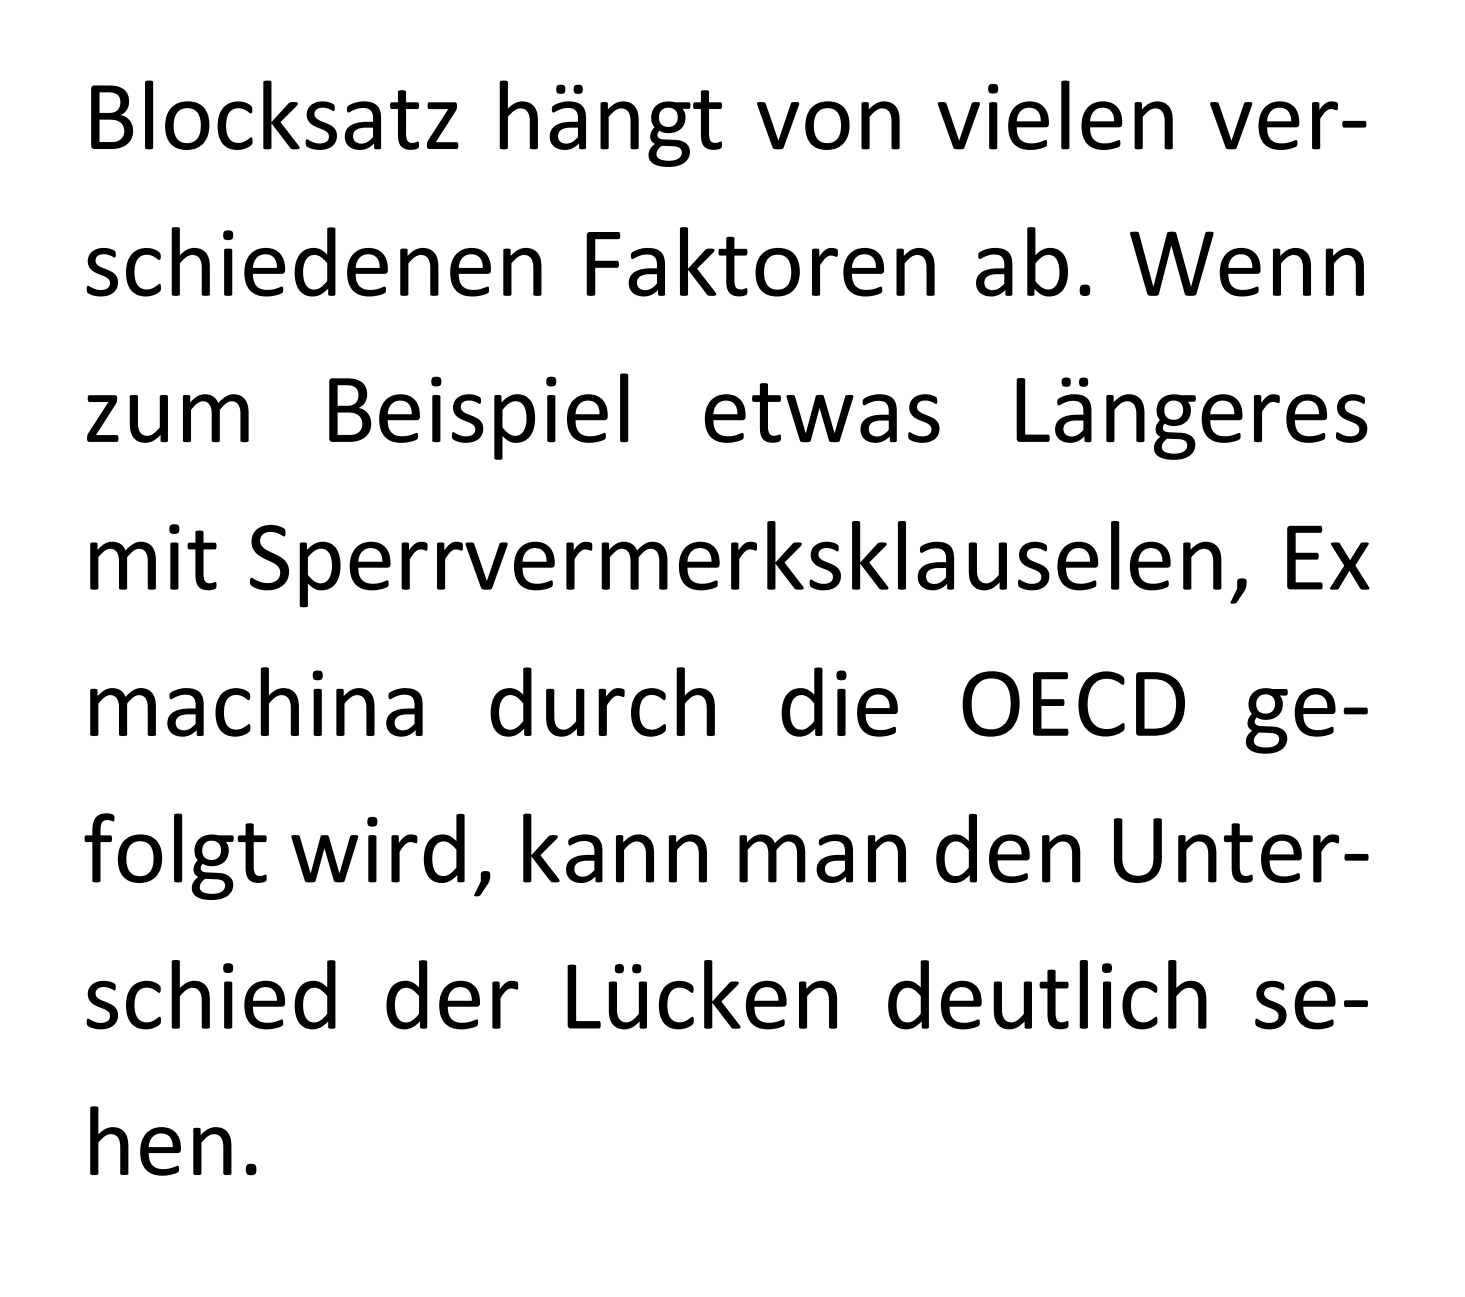
\includegraphics[width=.4\textwidth]{../assets/block-word.png}
    }
    ~ %add desired spacing between images, e. g. ~, \quad, \qquad, \hfill etc. 
      %(or a blank line to force the subfigure onto a new line)
    \subfloat[Textsatzprogramm, auch Typst]{
        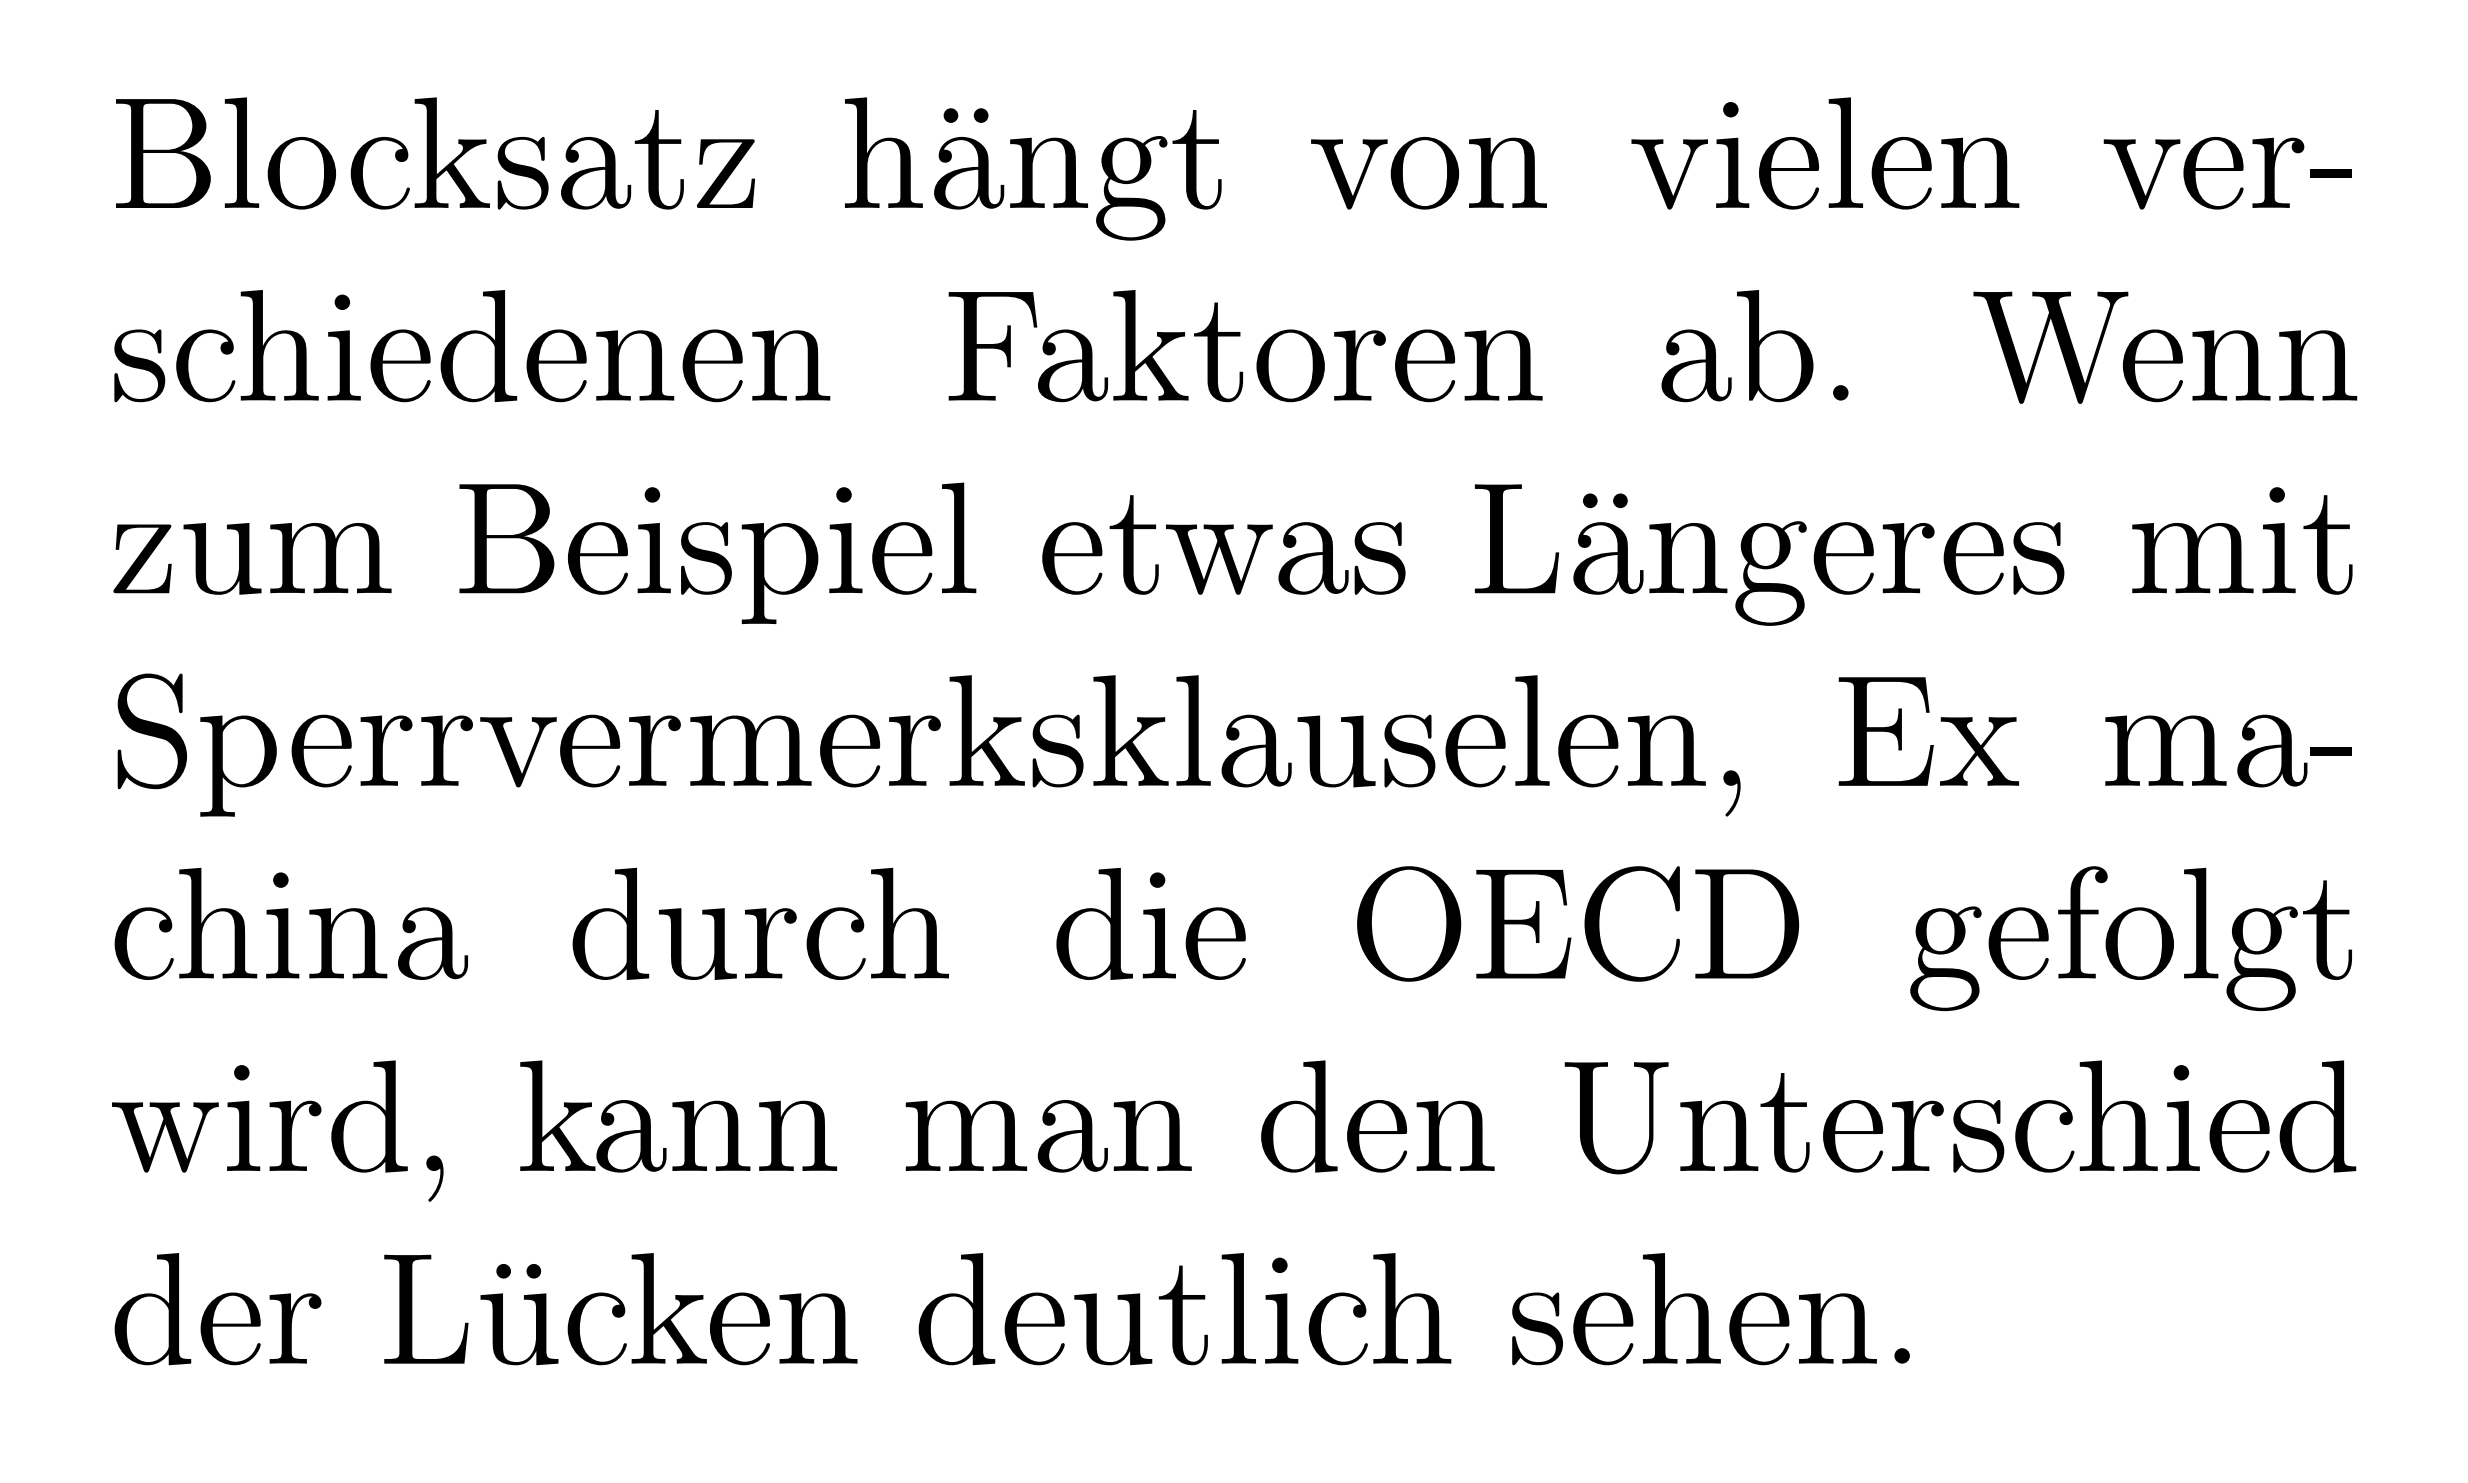
\includegraphics[width=.4\textwidth]{../assets/block-latex.png}
    }
    \caption{Qualitätsunterschied in Blocksatz und Silbentrennung: 
  Beim linken Absatz deutliche Unterschiede bei der Länge der Leerstellen.}
\end{figure}

\textbf{Effizient:} Viele Dokumente, wie Bücher einer Reihenausgabe oder wissenschaftliche Artikel, haben ein standardisiertes Layout. Dokumente in solchen Standard-Stilen zu formatieren, sollte für Nutzer\gender{}innen möglichst einfach sein. Gleichzeitig muss es einfach bleiben, später das Layout eines Manuskripts zu ändern, wenn der Text beispielsweise in einer anderen Reihe oder Zeitschrift erscheinen soll als ursprünglich geplant.

Nutzer\gender{}innen wollen sich beim Verfassen ihrer Texte aufs Schreiben konzentrieren, und nicht  ständig ihren Text formatieren müssen. Sie möchten sofort sehen, wie der aktuelle Text im fertigen Layout aussehen würde. Daher brauchen sie ein System, das das gewünschte Layout für beliebigen Inhalt möglichst automatisch umsetzt.

Hier hat Typst eine weitere große Stärke. Effizienz bei der Dokumenterstellung steht bei Typst im Vordergrund. Ein Layout, sobald einmal definiert, kann auf jeden beliebigen Inhalt angewendet werden. Dabei kann dieses Layout von der\gender{} Autor\gender{}in selbst oder einer\gender{} Designer\gender{}in gestaltet werden, oder auch als Vorlage beispielsweise von einer wissenschaftlichen Konferenz bereitgestellt werden. Die Layout-Befehle mischen sich dabei nicht mit dem Text, so dass auch nicht-technische Autor\gender{}innen nach minimaler Einweisung am Inhalt mitarbeiten können.

\textbf{Nutzerfreundlich:} Die meisten Schriftstücke werden von mehr als einer Person erstellt, entsprechend wollen Nutzer\gender{}innen in ihrer Textsatzsoftware mit anderen zusammenarbeiten, und das insbesondere auch gleichzeitig von verschiedenen Geräten aus. Darüber hinaus erwarten sie, dass das System generell einfach zu erlernen, ergonomisch zu bedienen und schnell ist. Sie wollen weder für jede Aufgabe ein Online-Tutorial zu Rate ziehen noch mehrere Sekunden warten, bis die Auswirkungen ihrer letzten Änderung zu sehen sind.

Werkzeuge sollten ihren Zweck erfüllen, statt sich in den Vordergrund zu rücken. Typst ist einfach zu erlernen, bleibt auch mit großen Dokumenten schnell, und selbst komplexe Layouts lassen sich damit leicht umsetzen.

\subsubsection*{Nachhaltigkeit \& Gesellschaft}

Schnelle Software, das heißt immer auch umweltfreundliche Software: Weniger Berechnungen verbrauchen weniger Strom und verschleißen weniger Festplatten. Weil Typst von Grund auf für Geschwindigkeit und Effizienz designt wurde, können hier signifikante Nachhaltigkeits-Vorteile realisiert werden, von denen die Nutzerbasis direkt profitiert. Zudem wird Typst, anders als beispielsweise LaTeX bei Overleaf,  nicht auf Remote-Servern, sondern direkt auf den Computern der Nutzer ausgeführt, was Datenverkehr im Internet und somit klimaschädliche Emissionen einspart.


Durch die starken kollaborativen Aspekte von Typst wird mehr Remotearbeit und Teamwork auch auf Entfernung ermöglicht. Der Trend zu mehr \cited{2} Hybrid- und Remotearbeit besteht bereits seit einer Weile, wurde aber durch die Pandemie deutlich beschleunigt. \cited{3} 47\% der von Envoy befragten US-Amerikaner\gender{}innen antworteten, dass sie sich wahrscheinlich nach einer anderen Stelle umsehen werden, wenn ihr\gender{}e Arbeitgeber\gender{}innen keine Hybridarbeit zulassen. Dieser Trend ist gesellschaftlich wünschenswert, da so eine flexiblere Familienplanung möglich wird, weniger gependelt wird und das Privatleben und der Beruf vereinbarer werden. Die Kollaborations-Features von beispielsweise InDesign sind einfach nicht mehr ausreichend für eine so dezentralisierte Erwerbsbevölkerung.

\section*{Wer?}
\subsection*{Kundensegmente}

Am Anfang sind Wissenschaftler\gender{}innen, Studierende (insbesondere in MINT-Fächern) und Universitäten unser wichtigstes Kund\gender{}innensegment. Mitglieder von Hochschulen müssen viele Texte verfassen, sei es zur Veröffentlichung von Artikeln oder bei Haus- und Abschlussarbeiten. \cited{4} Erfolgreiche Informatik-Professoren veröffentlichen zum Beispiel mehr als sechs Artikel pro Jahr. In der Wissenschaft wird generell eine hohe Layout-Qualität (auch von Formeln, Abbildungen, Referenzen etc.) erwartet. Meist verlangen Fakultät oder Herausgeber der Veröffentlichung zudem einen bestimmten Layoutstil. Da Wissenschaftler\gender{}innen fast immer im Team arbeiten (manchmal mit 5.154 Mitgliedern\cited{5}), steht eine reibungslose Zusammenarbeit im Mittelpunkt.

Die obigen Anforderungen bezüglich Satzqualität und verschiedenen Inhaltsbausteinen erfüllen bisherige Textverarbeitungen wie Word jedoch oft nur mangelhaft. LaTeX wiederum \cited{6}frustriert mit seiner hochkomplizierten Bedienung und langsamer Anzeige des Satzergebnisses viele seiner Benutzer\gender{}innen. Trotzdem ist es momentan aus den genannten Gründen die in der Wissenschaft verbreitetste Lösung.

Im wissenschaftlichen Segment sind dadurch immerhin schon viele Nutzer mit dem Paradigma des markupbasierten Textsatzes vertraut. Ein Wechsel zu Typst, das die Schwachstellen der etablierten Systeme überwindet, aber die Stärken der bisherigen Lösung erhält und ausbaut, wird somit leicht fallen. Hinzu kommt, dass Kund\gender{}innen in diesem Sektor durch die persönlichen Netzwerke der Gründer und ihrer Herkunft aus der Hochschul-Informatik einfach zu erreichen sind.


Im angepeilten Kundensegment sind die Zugewinne durch \glossary Netzwerkeffekte übrigens besonders stark ausgeprägt: Dadurch, dass in der Wissenschaft bei Veröffentlichungen sehr viel kollaboriert wird, werden alle der Co-Autor\gender{}innen Typst benutzen, sobald das Dokument dort angelegt wurde. Wir erwarten daher, dass sich die Software in einem Fachgebiet oder einer Lerngruppe rasch verbreitet. Dieser Effekt wird durch das angestrebte \glossary Freemium-Modell noch verstärkt, da auf diese Weise keine Barriere zum Einstieg in Typst bei zum Beispiel sparsamen Studierenden besteht, die für ein neues System nicht sofort Geld ausgeben möchten. Natürlich möchten wir mittelfristig auch zahlende Kunden gewinnen. Daher ist Kollaboration eine der Funktionen, die in der Gratis-Stufe des Freemium-Modells nur eingeschränkt zur Verfügung steht. So entsteht ein stärkerer Anreiz zum Abschluss eines Abonnements.


Zum Abschluss zwei Zahlen zur Größenordnung: Das Kundensegment besteht aus \cited{7}8 Mio. Wissenschaftler\gender{}innen und \cited{8}40 Mio. STEM-Studierenden weltweit, mit zusätzlichem Potential in anderen Fächern.

\subsubsection*{Expansionssegmente}

Da Typst eine Vielzahl von neuartigen nützlichen Funktionen bietet, streben wir nach unserem Markteintritt die Expansion in weitere Kundengruppen an.

Als erstes Expansionssegment bietet sich das Verlags- und Zeitungswesen an. Ein Buch oder eine Zeitung müssen hochwertig gesetzt sein und ihren typischen Stil aufweisen, sich dabei jedoch bei Bedarf jederzeit individuell anpassen lassen. An jeder Veröffentlichung arbeiten außerdem viele verschiedene Autor\gender{}, Grafiker\gender{}, Redakteur\gender{} und Setzer\gender{}innen. Bis dato werden dafür Desktop-Publishing-Programme wie InDesign mit InCopy und QuarkXPress verwendet, in denen Zusammenarbeit äußerst aufwändig ist. Typst verbessert kollaborative Prozesse bei gleichbleibender Satzqualität und ermöglicht schnellere Iteration am Text. Zu denken ist auch an Autor\gender{}innen im Self-Publishing, die selbst für einen hochwertigen Satz sorgen müssen und dazu bisher entweder viel Geld ausgeben oder komplizierte Programme erlernen müssen. Typst wird ihr Leben vereinfachen: Es bietet Vorlagen, die sofort für ein ansprechendes Ergebnis sorgen. Dieser Markt ist nicht zu vernachlässigen, denn \cited{9} 90\% der Autor\gender{}innen veröffentlichen im Self-Publishing.


Ein weiteres Expansionssegment sind die zahlreichen sonstigen Unternehmensgruppen, die ansprechend aussehende und dem eigenen Brandsystem entsprechende Printprodukte erzeugen wollen. Bisher wird dabei oft der Inhalt von einer Fachabteilungen erstellt und dann in zeitraubender manueller Arbeit von Design-Abteilungen umgesetzt. Mit Typst können Designer\gender{}innen ein arbeitssparendes System von wiederverwendbaren und leicht zu aktualisierenden Bausteinen erstellen, die von den Fachabteilungen mit minimalem Aufwand benutzt werden können. Liegen maschinenlesbare Daten vor, kann Typst dank seines integrierten Programmiersystems sogar eigenständig ganze Dokumente wie Serienbriefe oder Produktkataloge erstellen.

\newpage
\subsection*{Kundenbeziehungen}

Typst ist ein Werkzeug für kreativen Textsatz mit professionellem Anspruch. Der gemeinsame Nenner aller Beziehungen zu Kund\gender{}innen wird daher sein, Menschen zu helfen, ihre Textsatz-Bedürfnisse mit Typst zu erfüllen. Unsere Beziehungsstrategie hat deshalb drei Pfeiler: Befähigen, Inspirieren und Verbessern.

\subsubsection*{Befähigen}

Zunächst muss ein\gender{}e potentielle\gender{} Kund\gender{}in lernen, wie man Typst zur Dokumentenerstellung und -gestaltung verwenden kann. Wir sind uns bewusst, dass nicht alle Nutzer\gender{}innen aus unseren avisierten Kundensegmenten die Arbeit mit einem text- oder markupbasierten Textsatzsystem schon gewohnt sind. Daher ist es uns wichtig, viele didaktische Ressourcen wie spielerische Tutorials, typische Beispielaufgaben und ausführliche Erklärungen bereitzustellen. Nach solch einem sanften Einstieg in das Konzept realisiert ein\gender{}e Nutzer\gender{}in bald, wie leicht sich Typst den persönlichen Bedürfnissen anpassen lässt, während die umfangreiche Dokumentation hilft, tiefer in die detailreichen Features einzusteigen und in Kürze jedes sich stellende Layoutproblem eigenständig zu lösen.

Manchmal werden Nutzer\gender{}innen Fragen haben, die außerhalb des Rahmens unserer Dokumentation liegen. In einem leicht aus der Web-App zugänglichen Forum im Q\&A-Format können daher Fragen gestellt werden, die dann (auf Best-Effort-Basis) vom Typst-Team oder anderen Nutzer\gender{}innen beantwortet werden. Für zahlende Geschäftskunden soll zudem ein privater Support mit garantierter Antwortzeit eingerichtet werden.

\subsubsection*{Inspirieren}

Wir möchten Nutzer\gender{}innen fortlaufend inspirieren, eigene Projekte in Typst umzusetzen und die spannenden Möglichkeiten des Produkts immer ausgiebiger zu nutzen.

Zu diesem Zweck können zum Beispiel besonders gelungene oder ausgefallene Typst-Projekte von Nutzer\gender{}innen durch unsere Kanäle geteilt werden. Dabei entsteht ein für alle Parteien willkommener äußerer Werbeeffekt. Denn selbstverständlich erreichen so auch die Ersteller\gender{}innen dieser Projekte ein größeres Publikum.

Weiterhin werden Nutzer\gender{}innen davon profitieren, dass Tricks zu außergewöhnlichen oder eleganten Typst-Nutzungen geteilt werden. Solche kreativen Anwendungen regen im Idealfall andere Nutzer\gender{}innen zur Nachahmung an, wodurch auch sie sich enger mit Typst vertraut zu machen.

So wird nicht nur die Nutzung von Typst verstärkt und diversifiziert. Es stärkt auch die Brand Typst, weil sie kontinuierlich mit Kreativität und gut-aussehenden Print-Produkten verknüpft wird.

\subsubsection*{Verbessern}

Dank des Feedbacks von Nutzer\gender{} und Kund\gender{}innen kann das Wertangebot eines Produkts immer genauer auf die Kundenbedürfnisse abgestimmt werden. Deshalb legen wir besonderen Wert darauf, das Feedback der Nutzer\gender{}innen auf allen möglichen Kanälen anzunehmen. Natürlich trägt umgesetztes Feedback auch zur Kundenbindung bei.

Typst folgt dem Open-Core Modell, was heißt, dass Teile unserer Software quelloffen sind und öffentlich weiterentwickelt werden. Der wichtigste Bestandteil ist der \glossary Typst-Compiler, der Dateien in der Typst-Sprache in fertige Dokumente umwandelt. Technisch versierte Kund\gender{}innen können hier noch enger am Entwicklungsprozess teilhaben und ihre Nutzerperspektive einbringen. Wenn uns die entsprechenden Nutzungsrechte übereignet werden, ist es sogar möglich, dass Nutzer\gender{}innen eigene Funktionen zum Quellcode beitragen.


\newpage
\subsection*{Kanäle}

Grundsätzlich stehen Abonnement-Kund\gender{}innen im Zentrum unseres Geschäftsmodells. Dieses zahlende Kernkundensegment erzeugen wir durch zwei Ebenen von Kanälen. Über Awareness-Kanäle wecken wir zunächst Interesse bei potenziellen Kund\gender{}innen, indem wir ihnen zeigen, wie Typst ihre Probleme bei der Texterstellung lösen kann. Solche Kanäle schaffen Awareness. Durch sie ergibt sich eine erste Basis von Nutzer\gender{}innen, die Typst in der kostenfreien Variante verwenden. In einem zweiten Schritt möchten wir diese Nutzer\gender{}innen dann durch Conversion-Kanäle dazu bewegen, auf ein monatliches Abonnement umzusteigen.

\subsubsection*{Awareness}

Über Awareness-Kanäle kommunizieren wir unser Wertangebot an unsere Zielgruppen. Unser initiales Kundensegment ist die wissenschaftliche Gemeinschaft, die wir primär über die folgenden Kanäle zu erreichen planen:

\begin{itemize}
    \item \emph{Persönliches Netzwerk und Mundpropaganda:} Zu Beginn können wir Angehörige verschiedener Universitäten über persönliche und professionelle Kontakte mit Typst vertraut machen. Durch das starke Wertangebot empfehlen zufriedene Nutzer\gender{}innen Typst von sich aus an Kommiliton\gender{}innen und Kolleg\gender{}innen. Das ist insbesondere auch dann in ihrem eigenen Interesse, wenn sie mit diesen gemeinsam an Dokumenten arbeiten und dazu Typst verwenden.
    \item \emph{Wissenschaftliche Konferenzen:} Da unser initiales Kundensegment die wissenschaftliche Community ist, bietet es sich an über wissenschaftliche Konferenzen Aufmerksamkeit zu generieren. Das kann einerseits durch von uns eingereichte Veröffentlichungen über technische Aspekte von Typst geschehen, langfristig aber auch durch Partnerschaften, die die Einreichung von in Typst erstellen Arbeiten erleichtern (dazu später mehr).
    \item \emph{Social Media:} Über Social Media Plattformen verbreiten wir interessante Inhalte über Typst und dessen Entwicklung, um potenzielle Nutzer\gender{}innen initial mit unserem Wertangebot vertraut zu machen. Vor dem Launch laden wir hier dazu ein, unserer Mailingliste beizutreten, um Teil der geschlossenen Beta zu werden und anschließend einen dauerhaft kostenlosen Zugang zu Premium-Features zu erhalten.
    \item \emph{Performance Marketing:} So wie nahezu jedes andere Unternehmen werden auch wir bezahlte Anzeigen schalten, um Typst zu bewerben. 
\end{itemize}

\subsubsection*{Conversion}


Über \glossary Conversion-Kanäle stärken wir die Bindung von Kund\gender{}innen an das Produkt, damit Typst zu einem essenziellen Werkzeug ihrer Toolbox wird und so der Abschluss eines Premium-Abonnements der nächste logische Schritt ist. 

\begin{itemize}
    \item \emph{Mailing Liste:}  Vor dem Launch steht unsere E-Mail-Liste im Mittelpunkt. Wir nutzen sie, um andere Kanäle zu bewerben und die dortigen Abonnenten zum geschlossenen Beta-Test einzuladen. Dadurch können wir bereits Interessenten sammeln, während das Produkt noch in Entwicklung ist.
    \item \emph{Community Hub:} Später wird dann zunehmend ein Community-Hub in den Fokus rücken, auf dem Fragen gestellt und Inhalte (wie Vorlagen oder Tipps) geteilt werden können. Durch jede Diskussion über Typst ergeben sich Netzwerkeffekte, da immer zahlreichere Hilfsmaterialien und Vorlagen die Effizienz und Vielseitigkeit des Produkts steigern.
    \item \emph{Social Media:} Über Social Media lassen sich Ankündigungen von neuen Features, Tipps zur Nutzung von Typst und herausragende Community-Inhalte verbreiten. So können Nutzer\gender{}innen lernen, wie sie immer mehr aus Typst herausholen. Dieser Kanal ist besonders im Kontakt mit der kreativen Community effektiv, da diese hier sehr aktiv ist.
    \item \emph{Web Store:} Über den Web Store können Abonnements abgeschlossen werden. Hier findet also abschließend die Conversion zu zahlenden Nutzern statt.
    \item \emph{Direkter Kontakt:} Zu Organisationen wie Unternehmen oder Universitäten wird teilweise auch direkter Kontakt bestehen, um maßgeschneiderte Lösungen zu erstellen.
\end{itemize}


Schlussendlich sind der Web Store und direkter Kontakt zu uns die einzigen Wege unser Produkt zu erwerben. Alle anderen Kanäle sind darauf ausgerichtet, die Bindung von Kunden an das Produkt zu maximieren, um einen Abonnementabschluss möglichst wahrscheinlich zu machen.

\section*{Wie?}
\subsection*{Schlüsselaktivitäten}

Unsere Schlüsselaktivitäten unterteilen sich in solche Aktivitäten, die rein innerhalb des Unternehmens stattfinden, und solche, die auf Interaktion mit der Außenwelt abzielen.


Innerhalb des Unternehmens sollen zunächst die \glossary Typst-Sprache (sowie deren Compiler) und die Typst-Web-App fertig zu entwickelt werden, damit alle für das Wertangebot nötigen Funktionen vorhanden sind. Doch selbst nach dem initialen Launch wird Entwicklung eine wichtige Aktivität bleiben. Durch community-validierte Fortentwicklung kann die Nutzerfreundlichkeit des Web-Editors kontinuierlich gesteigert werden. Neue Funktionen im Compiler wiederum eröffnen weitere Gestaltungsmöglichkeiten für Dokumente.

Dazu kommt, dass Lernmaterialien, Dokumentationen, Beispiele und Vorlagen erstellt werden müssen. Wie im Abschnitt über Kundenbeziehungen erläutert, sind solche Materialien erforderlich, um Benutzer\gender{}innen an Typst heranzuführen und durch den schrittweisen Aufbau von Vertrautheit mit dem System die Conversion zur\gender{} zahlenden Abonnent\gender{}in wahrscheinlich zu machen.

Außerhalb des Unternehmens wollen wir unsere Beziehungen und Kanäle zu Nutzer\gender{}innen und anderen Mitgliedern unserer Kundensegmente unterhalten, sowie kontinuierlich neue Partnerschaften pflegen und schließen. Auch für unser erstes Kernkundensegment, die Wissenschaftsgemeinde, wird es zu Beginn wesentlich sein, ein Netzwerk aufzubauen, zu pflegen und zu nutzen. Hier soll eine Fakultät als Pilotkundin gewonnen werden. Mit dieser Kooperation können wir Benutzer\gender{}innen für Tests zur Validation des Wertangebots finden oder später allgemein Nutzer werben.

Die öffentlichen Awareness-Kanäle und die E-Mail-Liste müssen regelmäßig mit Content gemäß der Kundenbeziehungs-Strategie bespielt werden. Dies ist ein wichtiger Bestandteil unserer B2C-Marketing-Strategie. Hierfür kann man teils auf das oben generierte Material zurückgreifen, wir werden aber auch noch eigenes Material erstellen. Daneben wollen wir in diesem Aufgabenbereich noch Social Media Ads und anderes Performance Marketing konzipieren und betreuen.

Natürlich muss eine junge Community auch ausreichend betreut werden. Nutzer\gender{}innen, die sich am Diskurs um Typst beteiligen und unsere Kanäle nutzen, soll ein sicheres und freundliches Umfeld geboten und das Gefühl gegeben werden, dass wir bei Typst ihre Beiträge lesen und schätzen.

Die Priorisierung dieser Aktivitäten hängt von der weiteren Entwicklung unseres Produkts ab: Vor dem ersten Launch von Typst wollen wir vor allem an der Entwicklung und Erstellung von Lernmaterialien arbeiten, um danach zügig mit einem kundenfreundlichen System in den Markt einzutreten. Nach dem Launch geht es darum, die Nutzerbasis anwachsen zu lassen, weswegen der Fokus zu den nach außen gerichteten Netzwerk-, Marketing- und Communityarbeiten rückt.

\newpage
\subsection*{Schlüsselressourcen}


Die wichtigste Ressource von Typst ist das eigene geistige und intellektuelle Eigentum: Die Typst-Sprache und der Typst-Compiler bilden den Grundstein des Geschäftsmodells und enthalten zahlreiche originelle und innovative Lösungen. Obwohl der Typst-Compiler im Rahmen des \glossary Open Core-Modells öffentlich entwickelt wird, ist das enthaltene geistige Eigentum durch die genutzte Lizenz vor Wettbewerbern und Fremd-Kommerzialisierung geschützt. Neben der freien \glossary Copyleft-Lizenz wird der Compiler unter einer kommerziellen, proprietären Lizenz verfügbar sein, zum Beispiel für angepasste \glossary On-Premise-Installationen von Geschäftskund\gender{}innen.

\begin{figure}[h]
    \centering
    \subfloat[{Laurenz Mädje Sprachdesign \& \ Entwicklung}]{
        
\includegraphics[width=0.23\textwidth]{../assets/rund-l.png}
    }
    \quad %add desired spacing between images, e. g. ~, \quad, \qquad, \hfill etc. 
      %(or a blank line to force the subfigure onto a new line)
    \subfloat[{Martin Haug Entwicklung \& \ Business Development}]{
        
\includegraphics[width=0.23\textwidth]{../assets/rund-m.png}
    }
    \quad %add desired spacing between images, e. g. ~, \quad, \qquad, \hfill etc. 
    %(or a blank line to force the subfigure onto a new line)
    \subfloat[Co-Founder\gender{}in für Business Development]{
        
\includegraphics[width=0.23\textwidth]{../assets/rund-u.png}
    }
    \caption{Das Gründungsteam.}
\end{figure}

Um unser geistiges Eigentum im Markt zu platzieren, anzuwenden und weiterzuentwickeln, braucht Typst qualifizierte Software-Entwickler\gender{}innen, die ein technisches Produkt mit vielen unterschiedlichen Arbeitsbereichen und Fragestellungen abseits von Standardproblemen bearbeiten können. Die Arbeit von Laurenz Mädje und Martin Haug an den Prototypen von Compiler und Web-App zeigt, dass diese Positionen momentan gut besetzt sind.

Daneben sind für ein Produkt mit hohem Anspruch an die Nutzerfreundlichkeit auch immer User Experience (UX) Designer von hoher Bedeutung. Ein komplexes Produkt muss möglichst einfach und ergonomisch präsentiert werden. Die benötigte Expertise gilt nicht nur der graphischen Benutzeroberfläche der Web-App, sondern wird auch im Design der Typst-Sprache benötigt. Die Arbeit von Martin Haug im graphischen und Laurenz Mädje im Sprachdesign-Bereich war hier bisher erfolgreich, aber da Umfang und Bedeutung von UX-Aufgaben ständig zunehmen, werden wir immer wieder qualifizierte Designer, auch aus unserem eigenen Umfeld, für Auftragsarbeiten heranziehen.

Kurzfristig soll das Gründungsteam um eine\gender{} dritte\gender{} Co-Founder\gender{}in mit Expertise im Bereich Business Development ergänzt werden. Dieses zusätzliche Know-How wird uns helfen, Risikokapital und Förderung zu erhalten und mit unseren Kund\gender{}innenbeziehungen und Kanälen neue Nutzer\gender{}innen zu gewinnen. 

Durch seine Kundenbeziehungs-Strategie und ein visuell einheitliches Auftreten versucht Typst, eine Brand aufzubauen. Diese Brand wird zu einem wertvollen Tool, sobald Kund\gender{}innen sie künftig gedanklich mit Teamarbeit, Print und Kreativität assoziieren. Dann ist Typst als Markenname und Organisation schon so stark mit der gleichnamigen Markup-Sprache verbunden, dass es sogar für nichtkommerzielle Anbieter schwierig sein wird, online einen Konkurrenzdienst zur Typst Web-App anzubieten.

Typst-Nutzer\gender{}innen sind selbstverständlich auch dann eine Schlüsselressource für das Unternehmen, wenn sie keine zahlenden Abonnent\gender{}innen sind, weil sie, wenn sie kollaborativ arbeiten, einen Netzwerkeffekt entfalten und damit weitere neue Nutzer\gender{}innen auf unsere Plattform holen. Hinzu kommt, dass ein\gender{}e Nutzer\gender{}in nach einiger Zeit wahrscheinlich auch die Funktionen aus dem Abonnement benötigt und deshalb konvertieren wird.

Eine Schlüsselressource von Typst ist zu guter Letzt das zur Verfügung stehende Kapital. Mit mehr Kapital kann mehr Marketing betrieben werden, dies generiert dann wiederum mehr User. Um auf unkomplizierte Art Investment annehmen und dafür Anteile anbieten zu können, wird Typst als Kapitalgesellschaft gegründet. Typst möchte ein vertrauenswürdiger Geschäftspartner sein und deshalb eine Gesellschaft mit begrenzter Haftung (GmbH) werden. Dies erfordert eine gesetzlich festgelegte Stammeinlage in Höhe von 25.000 Euro.

Standortfaktoren für Typst sind vor allem, dass gute Akquisemöglichkeiten von weiterem qualifizierten Personal gegeben sind, außerdem das nötige Investmentkapital und universitäre Kunden. Berlin passt mit seinen drei international bekannten Exzellenz-Universitäten, hoher Attraktivität für junge, qualifizierte Professionals und dem wachsenden Risikokapital-Ökosystem gut zu diesen Anforderungen.


\newpage
\subsection*{Schlüsselpartner}

Am wichtigsten sind anfangs Partner, die uns Zugriff auf Finanzierung und neue Nutzer ermöglichen. Mit ihnen verstärken wir die Reichweite und Effektivität unserer Awareness-Kanäle.

Die Pilotfakultät wird zeigen, dass und wie Typst in der Praxis eingesetzt werden und reale Probleme lösen kann. Unsere Erfahrungen aus dem Pilotprojekt lassen wir sowohl zurück in die Entwicklung fließen als auch in unsere Kommunikation. Im Erfolgsfall dient die Pilotfakultät als eine Keimzelle für die Typst-Nutzung an Universitäten und deren Partnern.

Außerdem können unsere Mentoren (Nicolai Bull, PhD, wissenschaftlicher Mitarbeiter an der TU Berlin) und unser persönliches Umfeld (darunter Prof. Dr. Hartmut Haug, emeritierter Professor an der Universität Frankfurt) dabei helfen, Wissenschaftler\gender{}innen zu erreichen und als Nutzer\gender{}innen zu gewinnen. Besonders Wissenschaftler\gender{}innen mit großen Arbeitsgruppen möchten wir für Typst interessieren. Sie und ihre Gruppen sollen mit einem lebenslangen Abonnement angeworben werden. Mit ihrer Hilfe wird Typst auch international an Bekanntheit gewinnen.

In der ersten Aufbau-Phase benötigt Typst Kapital, um ein Produkt auf den Markt zu bringen. In der zweiten dann, um die Nutzerzahlen zu vergrößern. Für die Phase bis zum Marktstart streben wir daher auch ein Gründungsstipendium wie EXIST oder BSS an. So können der Lebensunterhalt der Gründer\gender{}innen und anfängliche Ausgaben finanziert werden. Für kapitalintensivere Akquise und Expansion wird später die Unterstützung eines Risikokapitalgebers äußerst hilfreich.

Eine der wichtigsten Partnerschaften von Typst müssen wissenschaftliche Journals und Konferenzen sein, die ja für die Kernkundengruppe von besonderer Bedeutung sind. Veranstalter\gender{} und Herausgeber\gender{}innen können eigene Vorlagen für ihre Autor\gender{}innen bereitstellen (die Vorlagen der wichtigsten Journals und Konferenzen wurden vorsorglich schon intern im Rahmen der Schlüsseltätigkeiten erstellt). Obwohl viele Konferenzen und Journals fertige PDFs als Einreichungen annehmen, fordern manche ein LaTeX- oder gegebenenfalls ein Word-Dokument, zum Beispiel in der Physik. Ein wichtiges Ziel einer Partnerschaft wäre es, für solche Zwecke die Abgabe im Typst-Format zu ermöglichen.

Das Wertangebot von Typst lässt sich durch Integrations-Partnerschaften in der Web-App weiter untermauern. Ein Beispiel für eine solche Integration wäre Mendely (ein Dienst zur Verwaltung von Literaturbibliotheken). Nutzer\gender{}innen würden in diesem Fall Inhalte direkt aus ihrer dortigen Bibliothek zitieren können, wobei vollautomatisch passende Referenzen erzeugt werden. Der Partnerdienst wird dabei direkt in die Typst App integriert. Die\gender{} Nutzer\gender{}in muss aber weiterhin auch Kunde des Partners sein, um die Integration vollumfänglich nutzen zu können. Solche Integrationen demnach sind von wechselseitigem Vorteil. Weitere Möglichkeiten für solche Partnerschaften wären Grammarly (fortgeschrittene englische Rechtschreib- und Stilprüfung), Wolfram (Analyse von mathematischen Ausdrücken) und Figma (direkter Import von stets aktuellen Vektorgrafiken).

Das Hosting der Web-Anwendung von Typst wird durch einen Cloud-Provider wie Amazon Web Services durchgeführt. Neben der Qualität der Plattform achten wir bei der Auswahl des Providers vor allem auf Nachhaltigkeitsaspekte wie Energieeffizienz und Anteil des nachhaltig erzeugten Stroms.

Schließlich könnte mit Font Foundries als Dienstleister und Partner die Brand und das Wertangebot gestärkt werden: Indem zahlenden Abonnenten exklusive Schriftarten von externen Designern für ihre Dokumente angeboten werden, wird ein zusätzlicher Anreiz zum Konvertieren geschaffen. Zudem ist so eine Partnerschaft effektives Marketing und stärkt die Brand von Typst als Hub und Werkzeug für Kreativität und Exzellenz im Print-Design.

\section*{Wie viel?}
\subsection*{Einnahmequellen}


Typst verfolgt ein Freemium-Modell, was heißt, dass ein Grundzugang zur Web-App kein Abonnement erfordert. Stattdessen muss ein\gender{}e Nutzer\gender{}in genau dann zur Kund\gender{}in werden, wenn er\gender{}sie mit mehr als zwei anderen Nutzer\gender{}innen an einem Projekt arbeiten oder mehr als fünf Projekte anlegen möchte. Außerdem sind Funktionen wie \glossary PDF/X-Compliance zur professionellen Druckproduktion nur für Abonennt\gender{}innen verfügbar.

Die Haupteinnahme-Quelle von Typst sind demzufolge die Abonnements der Kund\gender{}innen aus dem B2C-Bereich. Unsere Abonnements werden monatlich 10 € kosten, was ein typischer Preis für Software-as-a-Service Angebote ist und vergleichbar mit weit verbreiteten Angeboten wie Spotify Premium. Wenn die Kund\gender{}innen sich für ein Jahr an ihr Abonnement binden, wird zudem ein Rabatt gewährt, da wir sie so langfristig binden können und zuverlässigere Zahlungsströme erschließen. 

Die Konkurrenz verfolgt ebenfalls hauptsächlich ein Abo-Modell. Eine Lizenz für Microsoft Office und QuarkXPress lässt sich abweichend von uns auch mit einer Einzelzahlung erwerben, erlaubt dann aber keinen permanenten Zugriff auf Updates oder ein Cloud-Angebot. Der monatliche Abonnementpreis der Konkurrenten variiert dabei zwischen sieben (Microsoft Office mit Word) und 24 Euro pro Monat (Adobe InDesign), Overleaf liegt mit 14 Euro pro Monat im Mittelfeld. Bei manchen Anbietern sind Rabatte für Studierende und/oder andere Angehörige von Hochschulen verfügbar.

\begin{figure}[h]
  \centering
  \begin{tabular}{ | l | l | l | l | }
    \hline
    & Geschlossene Beta & Jahr 1 & Jahr 2 \\ \hline
    MAU & 500 & 6.000 & 80.000 \\ \hline
    Abonnent\gender{}innen & 0 & 300 & 4.000 \\ \hline
    Umsatz & 0€ & 15.000€ & 200.000€ \\ \hline
  \end{tabular}
  \caption{Nutzerentwicklungs und Umsatz-Ziele für die B2C-Vermarktung.}
\end{figure}


Wir erwarten, dass wir nach dem Abschluss eines Closed-Beta-Tests innerhalb eines Jahres von 500 auf 6.000 monatlich aktive User\gender{}innen (MAU) anwachsen, von denen 5\%, also 300, Abonnent\gender{}innen werden. Das ergibt einen Umsatz von 15.000 €. Das darauffolgende Jahr planen wir mit 80.000 MAUs und 4.000 Abonnements, abzuschließen und so einen Umsatz in Höhe von 200.000 € zu erzielen. Die Umsatzzahlen berücksichtigen, dass nicht alle der Benutzer von Januar an Abonnenten waren. Diese Planung legt eine fünfprozentige wöchentliche \cited{10} Wachstumsrate zu Grunde, die laut Paul Graham, Gründer des Y Combinator Accellerators, ein Ziel für ein junges SaaS-Startup sein sollte.

Eine weitere Einnahmequelle sind Volumenlizenzen im B2B-Vertrieb, zum Beispiel für Hochschulen und deren Organisationseinheiten. Dabei wird monatlich ein Betrag pro Nutzer\gender{}in abgerechnet, bei hohen Nutzerzahlen sind Rabatte verfügbar. Solchen Kund\gender{}innen wird gegen weitere Gebühr ein Premium-Support mit garantierter Rücklauf-Zeit offen stehen.

Mit Hilfe der doppelten Lizenzierung des Typst-Compilers wird außerdem möglich sein, Enterprise-Kunden aus den Expansionskundensegmenten, Typst (inklusive Web-App) für ihre eigenen Rechenzentren zu lizenzieren. Das dürfte attraktiv für Firmen sein, die besonders hohe Sicherheitsstandards für ihre internen Dokumente einhalten müssen oder den Typst-Compiler modifizieren wollen, ohne ihre Änderungen offenzulegen.

Zunächst benötigt Typst aber Kapital, um erfolgreich in den Markt zu starten. Hierfür wollen wir ein Gründungsstipendium wie EXIST oder BSS erhalten. In der Phase unmittelbar nach dem Markteintritt bestimmt die Menge des verfügbaren Kapitals maßgeblich, wie viele Early Adopter gewonnen werden können, die die Basis für das spätere Wachstum bilden. Risikokapital kann in der Anfangsphase also ausschlaggebend sein.

\newpage
\subsection*{Kostenstruktur}

Da das Geschäftsmodell von Typst darin besteht, innovative Technik auf den Markt zu bringen und zu verkaufen, also wertorientiert ist, entstehen die höchsten Kosten zunächst bei der Entwicklung dieser Technik. Dabei handelt es sich vor allem um Ausgaben für hochqualifizierte Software-Entwicker\gender{} und UX-Designer\gender{}innen. Für das dreiköpfige Gründungsteam fällt pro Person zunächst ein Betrag von 24000 Euro pro Jahr an, später entsprechend mehr.

Die zweite Kostensäule ist B2C-Marketing. Die Kosten sind hier größtenteils elastisch, da man mit mehr Geld eben entsprechend mehr Werbung schalten kann. Wir wollen den richtigen Betrag finden, um unsere Customer Acquisition Cost (CAC) zu minimieren. Langfristig streben wir eine CAC von unter 100 Euro an, insbesondere zu Anfang ist diese Obergrenze aber deutlich niedriger kalkuliert. Im ersten Jahr nach der geschlossenen Beta-Phase starten wir mit einem bescheidenen Marketing-Budget in Höhe von 2.000 Euro.

Hinzu kommen die Kosten für Hosting und Rechenzeit bei einem Cloud-Provider. In einer Musterrechnung für Amazon Web Services lassen sich die durchschnittlichen jährlichen Cloud-Kosten pro Nutzer\gender{}in (auch nicht abonnierte) nach oben mit 0,10 € pro Jahr abschätzen. Im Jahr nach der Beta beläuft sich dieser Posten also auf ca. 300 €. Dabei halten wir die Kosten nachhaltig gering: Dadurch, dass bei Typst besonders auf die Schnelligkeit geachtet wird, wird sowohl in der Cloud als auch bei der\gender{} Nutzer\gender{}in wenig Rechenzeit genutzt und Daten übertragen, was sowohl die Kosten als auch die Umweltauswirkungen minimiert, während die\gender{} Nutzer\gender{}in von einem schnellen Programm profitiert.

Für Ausrüstung fallen keine besonderen Kosten an, der bedeutenste Kostenpunkt sind hier Büromiete und perspektivisch Ausrüstung der Mitarbeiter\gender{}innen mit Firmen-Notebooks.

Zu guter Letzt fallen Kosten für Networking im wissenschaftlichen Bereich an. Hier entstehen verschiedene Posten wie Spesen, Fahrtkosten und Werbeartikel.

\section*{Ausblick}
\vspace{2mm}

Typst steht momentan ein knappes Jahr vor einer geschlossenen Beta und einem darauf folgendem generellen Markteintritt und damit als Unternehmen ganz am Anfang.

Obwohl Typst ein vielseitiges Produkt ist, wollen wir uns kurz- und mittelfristig auf den akademischen Markt konzentrieren, da die Vermarktung hier zunächst am einfachsten erscheint. Hier können wir unsere Unternehmensstrukturen und die Basis für eine spätere Kund\gender{}innengruppen-Expansion aufbauen.

Um erfolgreich im wissenschaftlichen Markt Fuß zu fassen, muss Typst in drei Jahren bei vielen Journals, die keine PDFs annehmen, als Abgabe-Format akzeptiert werden. Hier liegt ein Risiko, denn dafür müssen in den ersten Jahren Partnerschaften mit mehreren Herausgebern geschlossen werden. Daneben wollen wir nach Markteintritt, auch mit Feedback und Beteiligung der Nutzer\gender{}innen, Typst als Software weiterentwickeln, um die Anwendungszwecke für Textsatz im wissenschaftlichen Bereich vollständig abzudecken.

Von hier aus können wir eine Expansion in weitere Kund\gender{}innengruppen wie das Verlagswesen, die Design-Branche und Zeitungen anstoßen. Die Herausforderung ist in diesem Sektor, die Vorteile des markupbasierten Paradigmas von Typst effektiv zu vermarkten und die Web-App mit weiteren graphischen Tools zu ergänzen. Wenn dafür eine gute Strategie gefunden wird, kann Typst sich dank seinem Freemium-Modells und der branchenführenden Teamarbeitsfunktionen auch für diese Nutzer\gender{}innen eine gute Marktposition erarbeiten.

Mit effektivem Marketing können wir die Brand von Typst in Zusammenarbeit mit unseren Nutzer\gender{}innen mit Exzellenz im Print-Design, Kreativität und Teamarbeit assoziieren und sie so zu einer unserer Schlüsselressourcen machen und unserem geistigen Eigentum damit einen noch stärkeren Schutz zukommen lassen.

Laut unseren Wachstumsplanungen soll die Anzahl der monatliche aktiven User (MAU) im dritten Jahr nach dem allgemeinen Markteintritt im hohen sechsstelligen Bereich sein. Wir planen, über die ersten drei Jahre eine Conversion Rate von MAUs zu Abonennt\gender{}innen von 3 bis 5\% aufrechtzuerhalten. Dafür wird ein substantielles Marketingbudget nötig sein, dass auch aus Risikokapital stammen soll.

Das Team von Typst soll, sobald es die finanziellen Ressourcen zulassen, kontinuierlich ausgebaut werden. Mit festangestellten UX-Designer\gender{}innen, Sales-Representatives, Marketing-Expert\gender{}innen, und, nicht zuletzt, neuen Entwickler\gender{}innen, kann Typst sein Know-How und seine Agilität als Unternehmen deutlich steigern.

Langfristig soll Typst der neue Standard für akademischen und technischen Textsatz werden und in diesem Sektor allgemein für alle Veröffentlichungen akzeptiert werden. In den Branchen, die momentan von graphischen DPS-Systemen dominiert werden, streben wir ebenfalls langfristig an, Marktführer zu werden. \hfill {\color{eastern} ■}

\section*{Quellen}
\begin{tabular}{l p{.88\textwidth}}
    \textbf{↗} 1 & White, Karen. 2019. \emph{Publications Output: U.S. Trends and International Comparisons.} National Center for Science and Engineering Statistics: Alexandria, VA, USA. \url{https://ncses.nsf.gov/pubs/nsb20206/} \\
    \textbf{↗} 2 & Morar. 2015. \emph{The Flexible: friend or foe?} Vodafone: Berkshire, UK. \url{https://newscentre.vodafone.co.uk/press-release/974/} \\
    \textbf{↗} 3 & Smith, Jillian. 2021. \emph{Envoy survey finds employees want companies to embrace hybrid work and mandate COVID vaccines.} Envoy Blog: San Francisco, CA, USA. \url{https://envoy.com/blog/envoy-survey-finds-employees-want-companies-to-embrace-hybrid-work-and-mandate-covid-vaccines/} \\
    \textbf{↗} 4 & Newport, Cal. 2013. \emph{The Single Number that Best Predicts Professor Tenure: A Case Study in Quantitative Career Planning.} Study Hacks Blog. \url{https://www.calnewport.com/blog/2013/02/17/the-single-number-that-best-predicts-professor-tenure-a-case-study-in-quantitative-career-planning/} \\
    \textbf{↗} 5 & Castelvecchi, Davide. 2015. \emph{Physics paper sets record with more than 5,000 authors.} Nature: London, UK. \url{https://www.nature.com/articles/nature.2015.17567} \\
    \textbf{↗} 6 & Kanuff, Markus und Nejasmic, Jelica. 2014. \emph{An Efficiency Comparison of Document Preparation Systems Used in Academic Research and Development.} PLoS ONE 9 (12): San Francisco, CA, USA. \url{https://doi.org/10.1371/journal.pone.0115069} \\
    \textbf{↗} 7 & UNESCO. 2015. \emph{Facts and figures: human resources---From the UNESCO Science Report, Towards 2030.} \url{https://en.unesco.org/node/252277} \\
    \textbf{↗} 8 & World Bank. 2021. \emph{Higher Education.} Understanding poverty: Washington DC, USA. \url{https://www.worldbank.org/en/topic/tertiaryeducation#1} \\
    \textbf{↗} 9 & AskALLi Team. 2020. \emph{Facts and Figures about Self Publishing: The Impact and Influence of Indie Authors.} Alliance of Independent Authors Advice center: London, UK. \url{https://selfpublishingadvice.org/facts-and-figures-about-self-publishing-the-impact-and-influence-of-indie-authors/} \\
    \textbf{↗} 10 & Graham, Paul. 2012. \emph{Startup = Growth.} \url{http://www.paulgraham.com/growth.html} \\
\end{tabular}

{\footnotesize Alle Quellen wurden zuletzt am 15. Februar 2022 aufgerufen.}

\section*{Glossar}
\begin{tabular}{l p{.75\textwidth}}
\textbf{Blocksatz} & Satztechnik, bei der alle Zeilen in einem Absatz die volle Breite ausfüllen. Das wird durch Streckung und Stauchung der Abstände zwischen der Buchstaben und zuweilen durch leichte Verzerrung der Buchstaben selbst erreicht. Das Gegenstück zum Blocksatz ist der Flattersatz, bei dem die Lücken eine einheitliche Größe haben und die Zeilen unterschiedlich lang sind. \\
\textbf{Compiler} & Ein Programm, das Textdateien mit Inhalt in einer Markup- oder Programmiersprache in eine andere Datei umwandeln, im Falle von Typst in eine PDF oder ein Bild. \\
\textbf{Conversion} & Umwandlung von einer\gender{} Nutzer\gender{}in in eine\gender{} Kund\gender{}in. \\
\textbf{Copyleft} & Lizenz für quelloffene Software, die verlangt, dass sowohl bei Modifikationen der Software selbst als auch Programmen, die damit interagieren, der jeweilige Quellcode widerrum offengelegt wird. \\
\textbf{Freemium} & Monetarisierungsschema, bei dem eine Basis-Version des Produkts dauerhaft kostenlos genutzt werden kann, aber Zugriff für \emph{Premium}-Funktionen ein Abonnement abgeschlossen werden muss. \\
\textbf{Markup} & Markup sind Annotationen in einer Textdatei, die sich an den Computer richten und im finalen Dokument nicht enthalten sind. Stattdessen beeinflusst das Markup, wie der Inhalt im Ergebnis-Dokument präsentiert wird. Eine \textbf{Markup-Sprache} definiert, was für Markup verfügbar ist und welchen Effekt es hat. \\
\textbf{MINT} & Abkürzung für die Studiengänge in \textbf{M}athematik, \textbf{I}nformatik, \textbf{N}aturwissenschaften und \textbf{T}echnik. \\
\textbf{Netzwerkeffekte} & Ein Effekt, bei dem sich der Wert und damit die Attraktivität eines Produkts mit steigender Anzahl von Nutzer\gender{}innen erhöht. \\
\textbf{On-Premise} & Software, die nicht in der Cloud, sondern direkt auf dem Server der\gender{} Kund\gender{}in installiert ist. \\
\textbf{Open Core} & Geschäftmodell, bei dem ein zentraler Teil der Software, auf der das Geschäftsmodell aufbaut, quelloffen verfügbar ist. Dadurch wird der Nutzer\gender{}innenkreis stärker in die Entwicklung eingebunden und die Bildung eines \emph{Ökosystems} rund um das Produkt wird gefördert. \\
\textbf{PDF/X} & Spezieller PDF-Standard für die Druckproduktion. PDF/X-Dateien erlauben einen professionellen Druck mit präziser Farbwiedergabe. \\
\end{tabular}

\end{document}
